\documentclass[12pt]{article}
\usepackage[utf8]{inputenc}
\usepackage[russian]{babel}
\usepackage{graphicx}
\usepackage{listings}
\usepackage{indentfirst}
\usepackage{color}
\usepackage{multirow}
\usepackage{bm}

\definecolor{dkgreen}{rgb}{0,0.6,0}
\definecolor{gray}{rgb}{0.5,0.5,0.5}
\definecolor{ltgray}{rgb}{0.95,0.95,0.95}
\definecolor{mauve}{rgb}{0.58,0,0.82}
\newcommand{\rot}{\mathop{\rm rot}\nolimits}
\renewcommand{\lstlistingname}{Листинг}
\lstset{ %
  language=Python,                % the language of the code
  basicstyle=\footnotesize\ttfamily,           % the size of the fonts that are used for the code
%  numbers=left,                   % where to put the line-numbers
%  numberstyle=\tiny\color{gray},  % the style that is used for the line-numbers
%  stepnumber=2,                   % the step between two line-numbers. If it's 1, each line 
                                  % will be numbered
%  numbersep=5pt,                  % how far the line-numbers are from the code
  backgroundcolor=\color{ltgray},      % choose the background color. You must add \usepackage{color}
  showspaces=false,               % show spaces adding particular underscores
  showstringspaces=false,         % underline spaces within strings
  showtabs=false,                 % show tabs within strings adding particular underscores
  %frame=single,                   % adds a frame around the code
  rulecolor=\color{black},        % if not set, the frame-color may be changed on line-breaks within not-black text (e.g. comments (green here))
  columns=fixed,
  tabsize=2,                      % sets default tabsize to 2 spaces
  captionpos=b,                   % sets the caption-position to bottom
  breaklines=true,                % sets automatic line breaking
  breakatwhitespace=false,        % sets if automatic breaks should only happen at whitespace
%  caption=Valalala,                   % show the filename of files included with \lstinputlisting;
                                  % also try caption instead of title
  keywordstyle=\color{blue},          % keyword style
  commentstyle=\color{gray},       % comment style
  stringstyle=\color{dkgreen},         % string literal style
  escapeinside={\%*}{*)},            % if you want to add LaTeX within your code
  morekeywords={*,...},              % if you want to add more keywords to the set
  deletekeywords={...}              % if you want to delete keywords from the given language
}


\title{Сравнение схем расщепления для нестационарного уравнения Стокса}
\author{Виктор Борисов}

\begin{document}

\maketitle

\section{Задача}
Нестационарное уравнение Стокса описывает течение несжимаемой жидкости в области $\Omega$ с границей $\Gamma$:
\begin{equation}
\frac{\partial {\bm u}}{\partial t} -\Delta {\bm u} + \nabla p = {\bm f}({\bm x}), \quad {\bm x} \in \Omega,
\end{equation}
\begin{equation}
\nabla\cdot{\bm u} = 0, \quad {\bm x} \in \Omega,
\end{equation}
\begin{equation}
{\bm u} = {\bm g}({\bm x}), \quad {\bm x} \in \Gamma,
\end{equation}
где ${\bm u}({\bm x})$ - скорость, $p({\bm x})$ - давление и ${\bm f}({\bm x})$ - внутренний источник движения. В двумерной задаче ${\bm x}=(x_1, x_2)$, остальные векторные величины задаются аналогично: ${\bm u}=(u_1, u_2)$, ${\bm f}=(f_1, f_2)$, ${\bm g}=(g_1, g_2)$.

Рассматривается тестовая двумерная задача о течении в каверне с подвижной верхней границей. Подвижная верхняя граница означает, что вектор скорости на ней имеет ненулевое значение. Задача решается в безразмерных величинах на единичном квадрате $\Omega$ (рис. \ref{fg:cavity}), c границей $\Gamma=\Gamma_1 \cup \Gamma_2$, где на верхней границе $\Gamma_1$ скорость принимает значения ${\bm u}=(1, 0)$, в остальной части $\Gamma_2$ поставлено условие неприлипания и непротекания ${\bm u}=(0, 0)$.

\begin{figure}
	\begin{center}
		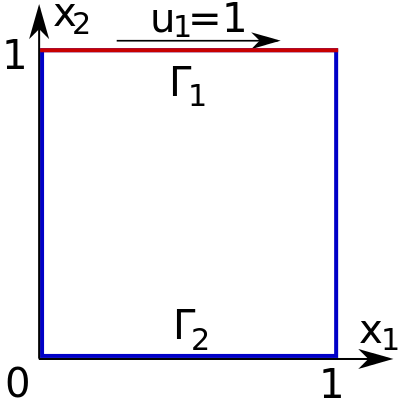
\includegraphics[width=200px]{pics/cavity400}
		\caption{Тестовая область с подвижной верхней границей.}
		\label{fg:cavity}
	\end{center}
\end{figure}

\section{Схемы}
Для решения использовано сочетание конечных элементов Тейлора-Худа.
Используются схемы с объединенным пространством неизвестных (неявная, Кранка-Николсона) и схемы с расщеплением (Дугласа-Рекфорда, Письмана-Рекфорда, локально-сбалансированная).
В схемах расщепления применяется операторы:
\begin{equation}
Nu = -\Delta u,
\end{equation}
\begin{equation}
Pu = \nabla p, 
\end{equation}
при условии $\nabla\cdot u = 0$.

\subsection{Неявная схема}
Обозначается IM.
\begin{equation}
\frac{u^{n+1}-u^n}{\tau} - \Delta u^{n+1}+\nabla p^{n+1}=0,
\end{equation}
\begin{equation}
\nabla \cdot u^{n+1}=0.
\end{equation}
\begin{figure}
	\begin{center}
		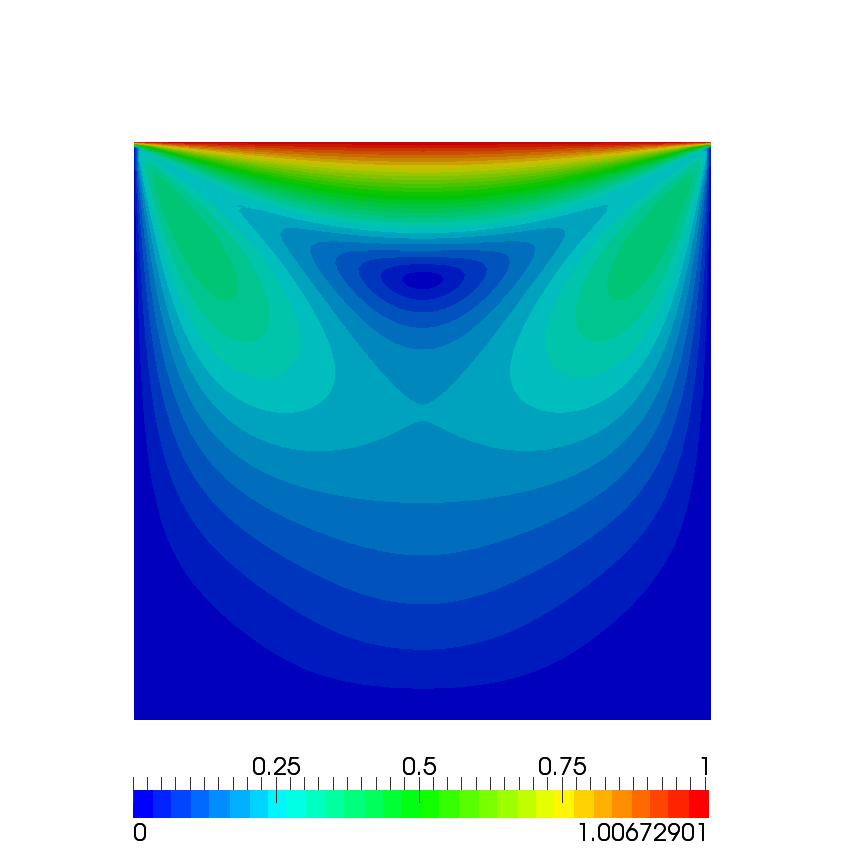
\includegraphics[width=400px]{pics/implicit}
		\caption{Неявная схема.}
		\label{fg:velocity-implicit}
	\end{center}
\end{figure}

\subsection{Схема Кранка-Николсона}
Обозначается CN.
\begin{equation}
\frac{u^{n+1}-u^n}{\tau} - \Delta \frac{u^{n+1}+u^n}{2}+\nabla \frac{p^{n+1}+p^n}{2}=0,
\end{equation}
\begin{equation}
\nabla \cdot \frac{u^{n+1}+u^{n}}{2}=0.
\end{equation}

\begin{figure}
	\begin{center}
		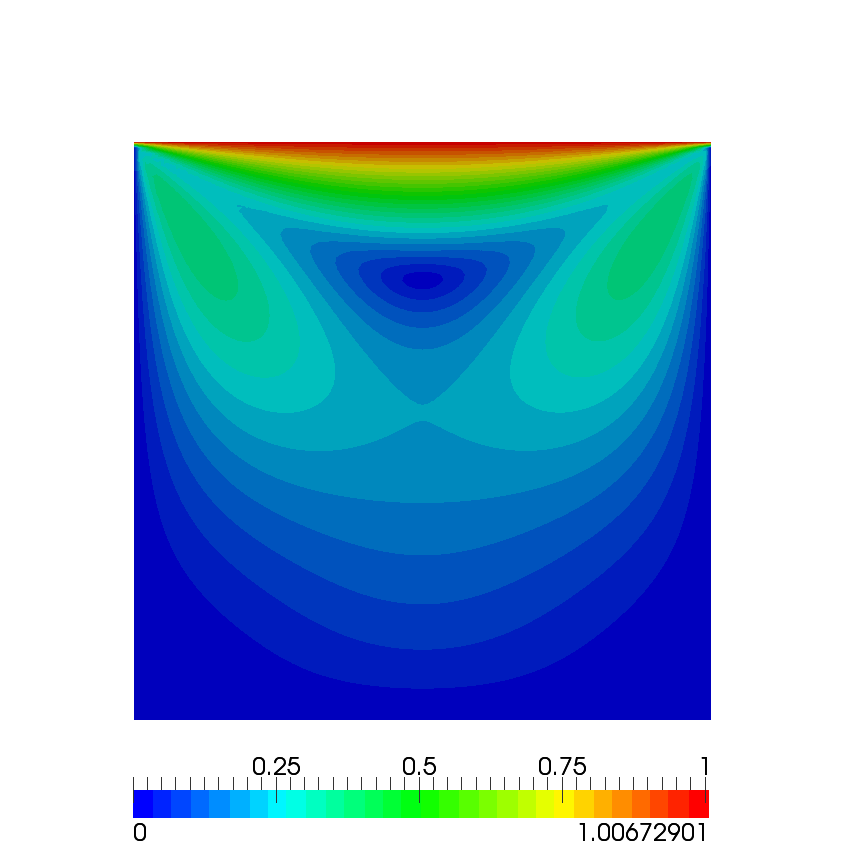
\includegraphics[width=400px]{pics/cn}
		\caption{Схема Кранка-Николсона.}
		\label{fg:velocity-cn}
	\end{center}
\end{figure}

\subsection{Схема расщепления Дугласа-Рекфорда}
Обозначается DR.
\begin{equation}
\frac{u^{n+\frac{1}{2}}-u^n}{\tau} + Nu^{n+\frac{1}{2}}+Pu^n=0,
\end{equation}
\begin{equation}
\frac{u^{n+1}-u^n}{\tau} + Nu^{n+\frac{1}{2}}+Pu^{n+1}=0.
\end{equation}

\begin{figure}
	\begin{center}
		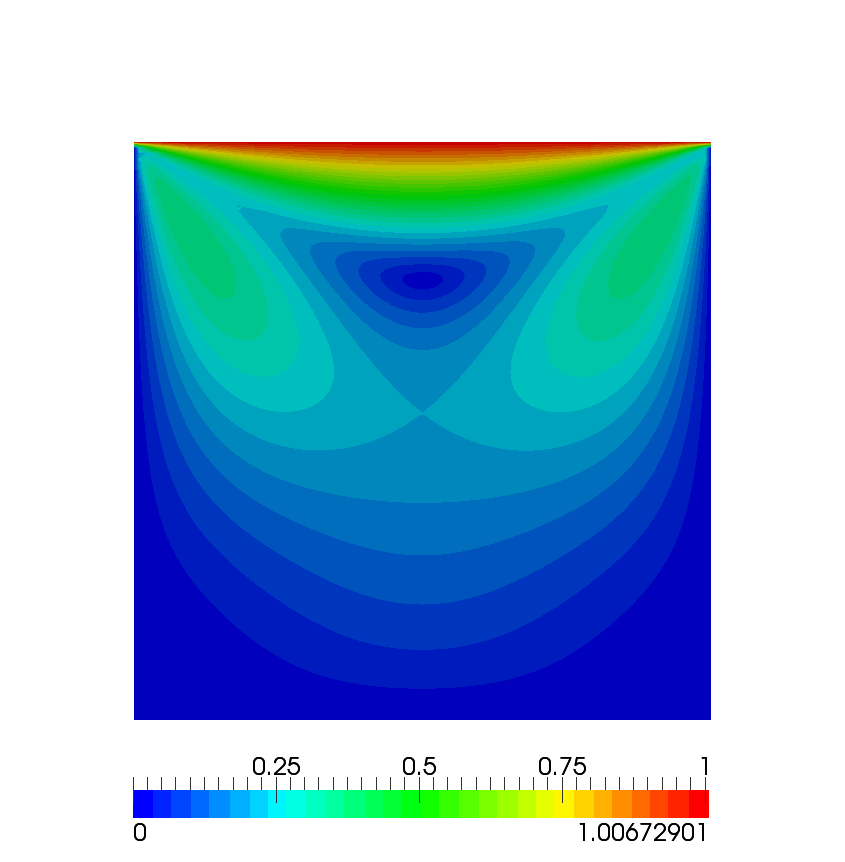
\includegraphics[width=400px]{pics/dr}
		\caption{Схема расщепления Дугласа-Рекфорда.}
		\label{fg:velocity-dr}
	\end{center}
\end{figure}

\subsection{Локально-сбалансированная схема расщепления}
Обозначается LB.
\begin{equation}
\frac{u^{n+\frac{1}{2}}-u^n}{\tau} + Nu^{n+\frac{1}{2}}=0,
\end{equation}
\begin{equation}
\frac{u^{n+1}-u^{n+\frac{1}{2}}}{\tau} + Pu^{n+1}=0.
\end{equation}
\begin{figure}
	\begin{center}
		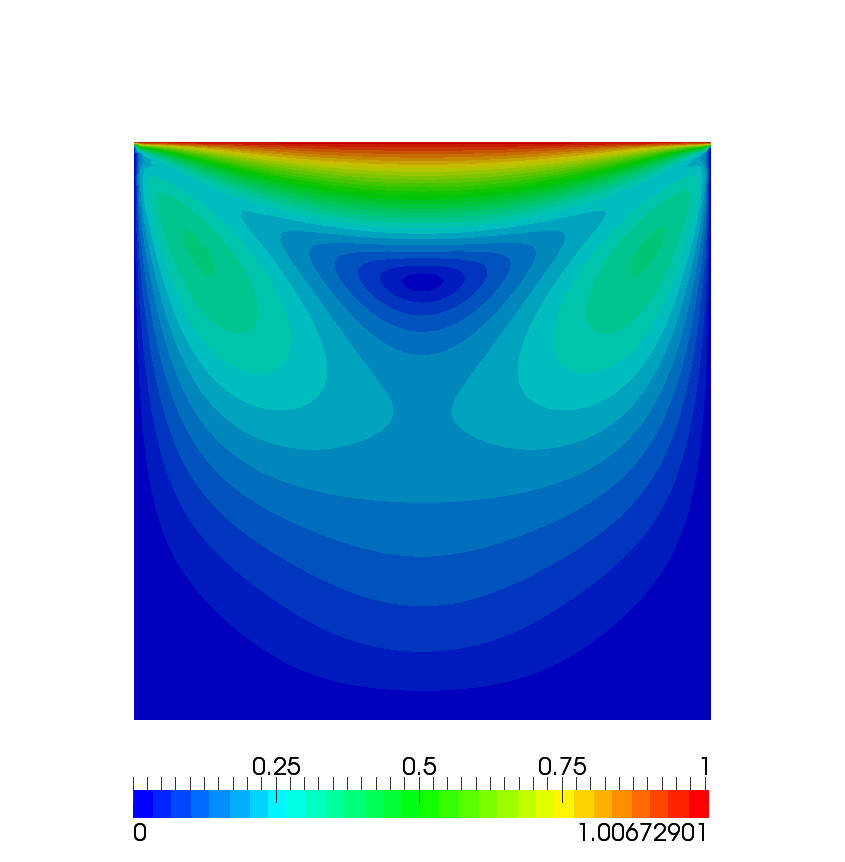
\includegraphics[width=400px]{pics/lb}
		\caption{Локально-сбалансированная схема расщепления.}
		\label{fg:velocity-lb}
	\end{center}
\end{figure}

\subsection{Схема расщепления Письмана-Рекфорда}
Обозначается PR.
\begin{equation}
\frac{u^{n+\frac{1}{2}}-u^n}{\tau/2} + Nu^{n+\frac{1}{2}}+Pu^n=0,
\end{equation}
\begin{equation}
\frac{u^{n+1}-u^{n+\frac{1}{2}}}{\tau/2} + Nu^{n+\frac{1}{2}}+Pu^{n+1}=0.
\end{equation}
\begin{figure}
	\begin{center}
		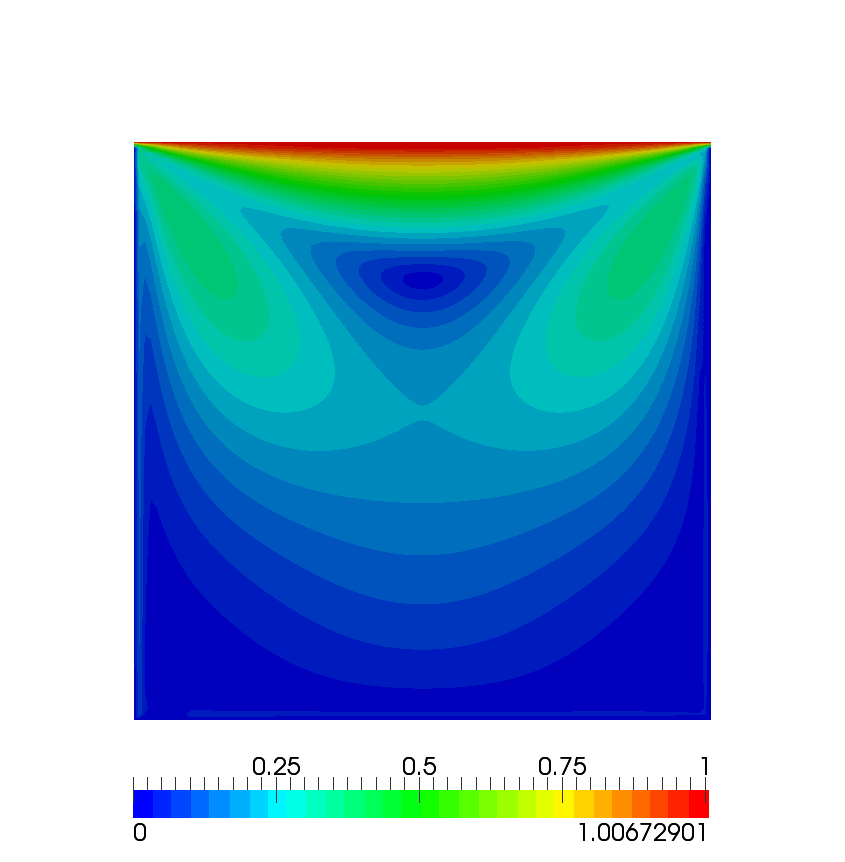
\includegraphics[width=400px]{pics/pr}
		\caption{Расщепление Письмана-Рекфорда.}
		\label{fg:velocity-pr}
	\end{center}
\end{figure}

\section{Результаты}
\begin{table}
    \begin{center}
	\begin{tabular}{|c|c|c|c|}
	    \hline	
	     & 25 & 50 & 100 \\
	    \hline	
	    IM & 38.59 & 239.46 & 1805.2 \\
	    \hline
	    CN & 40.77 & 244.16 & 1853.7 \\
	    \hline
	    DR & 39.12 & 197.86 & 1123.4 \\
	    \hline
	    PR & 38.96 & 198.43 & 1082.6 \\
	    \hline
	    LB & 37.39 & 192.17 & 1085.4 \\
	    \hline
	\end{tabular}	
	\caption{Зависимость времени выполнения различных схем от размера сетки.}
	\label{tb:time1}	 
	\end{center}
\end{table}	


\begin{table}
    \begin{center}
	\begin{tabular}{|c|c|c|c|}
	    \hline	
	     & 25 & 50 & 100 \\
	    \hline	
	    IM & 26.54 & 120.96 & 715.83 \\
	    \hline
	    CN & 27.50 & 126.20 & 751.61 \\
	    \hline
	    DR & 37.60 & 152.08 & 730.44 \\
	    \hline
	    PR & 35.39 & 152.55 & 833.39 \\
	    \hline
	    LB & 32.25 & 147.74 & 702.46 \\
	    \hline
	\end{tabular}	
	\caption{Зависимость времени выполнения различных схем от размера сетки для двух процессоров.}
	\label{tb:time2}	 
	\end{center}
\end{table}	

В таблице \ref{tb:time2} приведены сравниваемые схемы и их время работы после параллельного запуска на двух процессорах.
На рис. \ref{fg:slice1},  \ref{fg:slice199} приведены графики магнитуды скорости в разрезе $x=0.5$. Также в приложении есть видеофайл oscilate.avi, где видны колебания в методе Письмана-Рекфорда. Локально-сбалансированная схема не совпадает с другими схемами.

\begin{figure}
	\begin{center}
		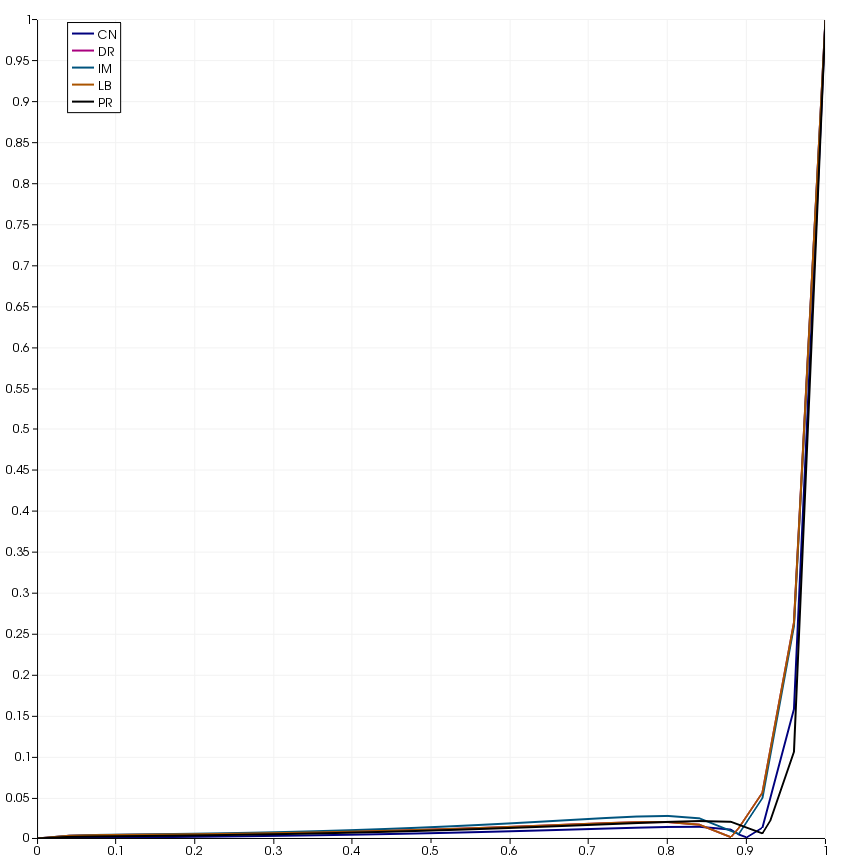
\includegraphics[width=400px]{pics/slice1}
		\caption{Распределение магнитуды скорости в разрезе $x=0.5$ первый временной слой.}
		\label{fg:slice1}
	\end{center}
\end{figure}

\begin{figure}
	\begin{center}
		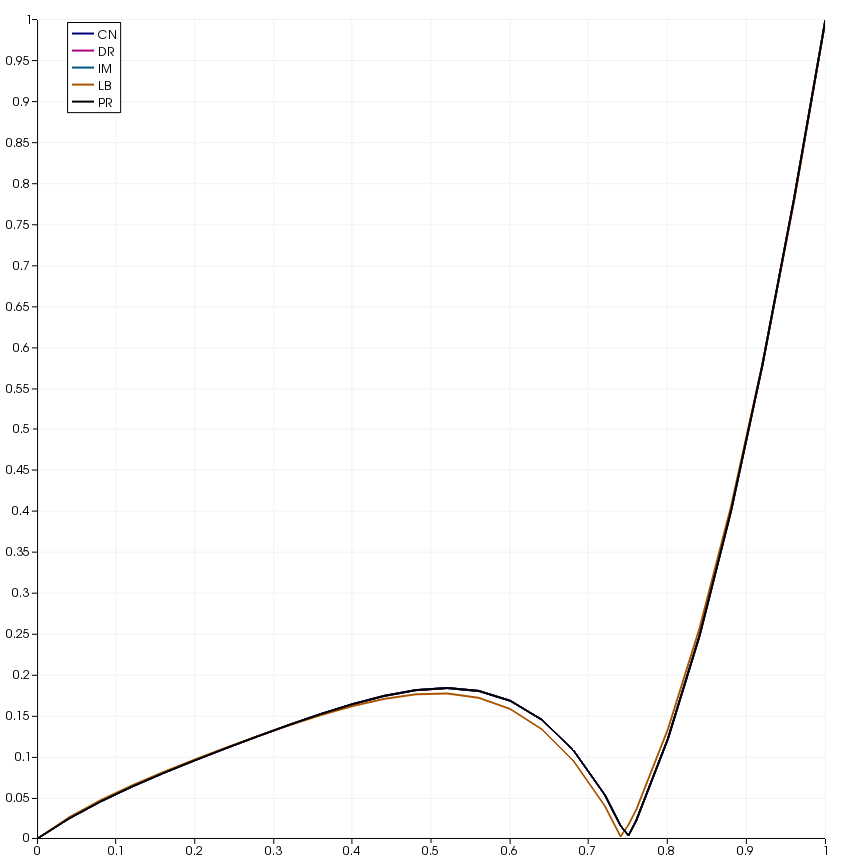
\includegraphics[width=400px]{pics/slice199}
		\caption{Распределение магнитуды скорости в разрезе $x=0.5$ последний временной слой.}
		\label{fg:slice199}
	\end{center}
\end{figure}


\end{document}